% =====================================================================================
%  Section 4.5 — What can the shield not reach?
%  Self-contained. Nothing to \input.
%
%  PREAMBLE (already in main.tex): graphicx, booktabs, multirow, threeparttable
%  ASSET: figures/fig_culprits.pdf
%    Regenerate:  PYTHONPATH=. python -m experiments.make_fig_culprits
%
%  TWO THINGS NOT TO EDIT AWAY:
%   (1) The culprit categories OVERLAP -- base is 71+17+36 = 124 attributions over 99 collided
%       episodes. Any phrasing implying the columns partition the collisions is wrong, and the
%       figure is grouped rather than stacked for the same reason.
%   (2) The arm-link improvement (17 -> 8) has OVERLAPPING Wilson intervals and is stated as
%       suggestive. The gripper result (71 -> 0 across 360 shielded episodes) is not in doubt.
%       Do not let the two be read at the same confidence.
% =====================================================================================

\section{What Can the Shield Not Reach?}\label{sec:res:scope}

The shield reduces collisions to 13.3\% but not to zero. This section identifies what the residual
consists of, using per-body collision attribution recovered from the evaluation logs. Contacts
attributed to other scene objects are excluded throughout: that category fires on every episode of
every condition, including collision-free ones, because an obstacle resting on its supporting
surface registers a permanent contact.

\begin{table}[htbp]
\centering
\begin{threeparttable}
\caption[Residual collisions by culprit body]{%
  Per-body attribution of collisions. Counts are episodes out of $n = 120$ in which the named body
  was implicated. Categories are not mutually exclusive, so a row need not sum to its collided
  count.\tnote{a}}
\label{tab:culprits}
\begin{tabular}{lrrrrr}
\toprule
\textbf{Policy} & \textbf{Episodes} & \textbf{Collided} & \textbf{Gripper} & \textbf{Arm link}
  & \textbf{Held object} \\
\midrule
Base, no shield        & 120 & 99 & 71          & 17 & 36 \\
Base + shield          & 120 & 16 & \textbf{0}  & 15 & \phantom{0}0 \\
\addlinespace[2pt]
Round 1, no shield     & 120 & 23 & \phantom{0}7 & 13 & \phantom{0}9 \\
Round 1 + shield       & 120 & 10 & \textbf{0}  & \phantom{0}8 & \phantom{0}1 \\
\addlinespace[2pt]
Round 2, no shield     & 120 & 21 & \phantom{0}8 & \phantom{0}8 & \phantom{0}7 \\
Round 2 + shield       & 120 & 11 & \textbf{0}  & \phantom{0}9 & \phantom{0}0 \\
\bottomrule
\end{tabular}
\begin{tablenotes}[flushleft]\footnotesize
\item[a] For example the base row records 124 attributions across 99 collided episodes, because a
  single episode may implicate more than one body.
\end{tablenotes}
\end{threeparttable}
\end{table}

\begin{figure}[htbp]
  \centering
  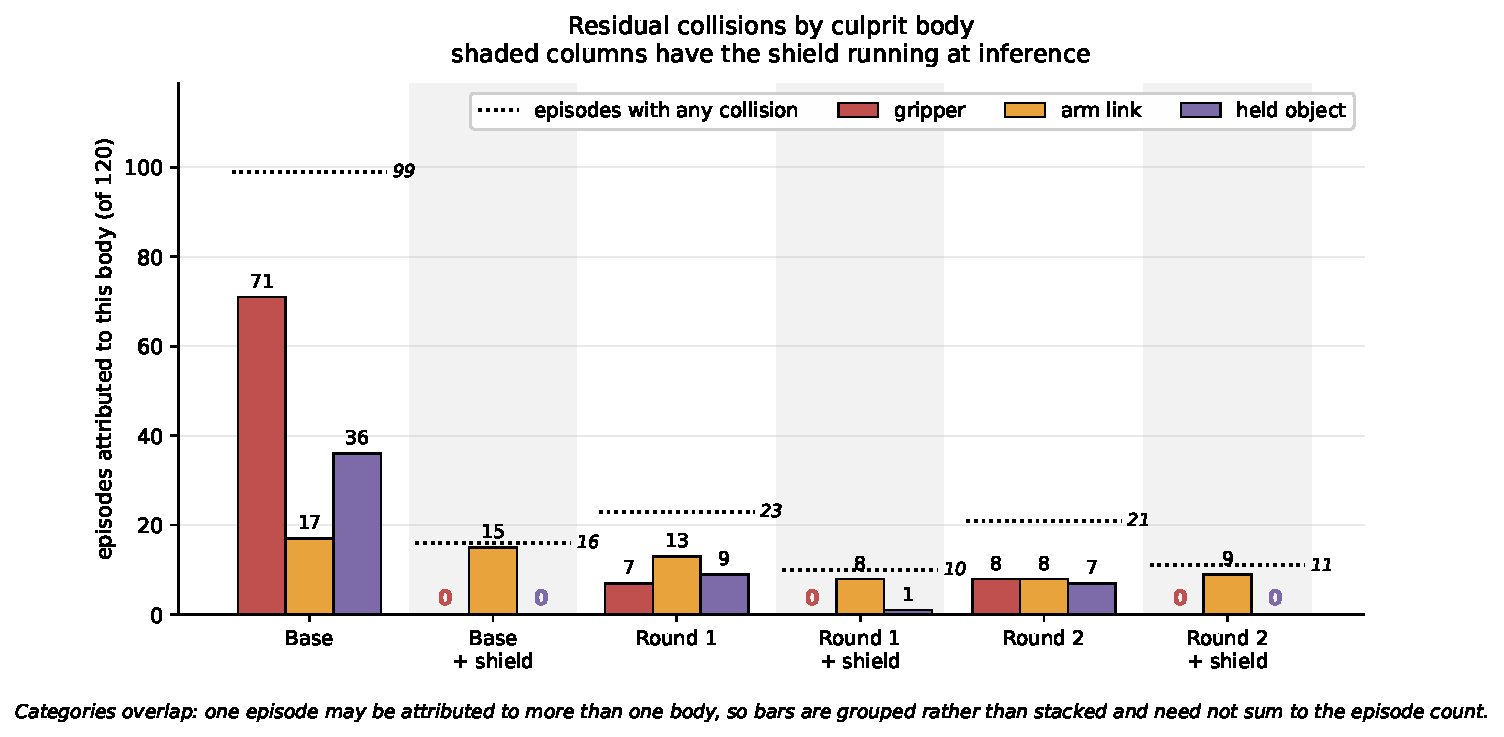
\includegraphics[width=\linewidth]{figures/fig_culprits.pdf}
  \caption[Collision attribution by body across conditions]{%
    What the shield reaches. The end-effector channel is eliminated wherever the shield is running
    (shaded columns): zero gripper collisions across all 360 shielded episodes. Arm-link contacts
    survive it almost unchanged. Bars are grouped rather than stacked because the categories
    overlap, and the dotted line marks the number of episodes with any collision at all.}
  \label{fig:culprits}
\end{figure}

\paragraph{The shield eliminates the end-effector channel completely.}
Gripper collisions fall from 71 to zero, and across all 360 shielded episodes there is not a single
one. Of the 16 residual collisions in the shielded baseline, 15 involve an arm link.

\paragraph{The residual is a fidelity limit, not a scope limit.}
Arm links are not absent from the barrier: links three to seven and the hand are constrained
(Section~\ref{sec:barrier}). But they are represented far more coarsely than the end-effector ---
three point samples per link carrying a single sphere radius, against three fitted spheres for the
hand and fingers. More importantly, an arm link's velocity is not the quantity the quadratic
program optimises. The program solves for an end-effector velocity and infers link motion through a
damped Jacobian pseudo-inverse, so the constraint is enforced against a \emph{predicted} link
velocity that diverges from the realised one wherever the inverse is ill-conditioned or the
controller's null-space motion differs from the minimum-norm solution.

The pattern in Table~\ref{tab:culprits} is therefore the expected one: collisions are eliminated
exactly where the barrier's model of the robot is precise and its velocity is the controlled
variable, and they persist where the model is coarse and the velocity is estimated. The corollary
for reading Section~\ref{sec:res:internalise} still holds --- the distilled policy's shield-free
figure is within a few points of what its teacher actually achieved, not a degraded approximation
of a perfect one --- but the teacher's own ceiling is set by approximation error in the constraint,
not by an absence of authority.

\paragraph{A second transfer channel.}
Arm-link collisions fall from 17 to 8 between the base and twice-distilled policies, while the
shielded baseline --- with the arm-link constraints active --- still shows 15. The improvement is
therefore not inherited from the barrier's own arm-link performance, which is worse than the
student's. It must come instead from the selection criterion: demonstrations were retained only if
nothing at all was displaced, arm links included, and the student learned that. Safety appears to
transfer through two distinguishable channels --- imitation of the filter's corrections where the
filter has authority, and outcome selection where it does not.

This second channel is stated with less confidence than the first. As proportions, 17/120 against
8/120 is 14.2\% [9.0, 21.5] versus 6.7\% [3.4, 12.6]; those Wilson intervals overlap, so the
arm-link trend is suggestive rather than established. The gripper result is not in doubt.

\paragraph{Independent corroboration.}
A separate experiment measured the end-effector's closest approach to the obstacle during level-II
episodes that were scored as collisions. The minimum was 0.231\,m against a barrier radius of
0.15\,m: the end-effector never came close, yet the episode collided. Together with the attribution
table and the inert guided-sampling result of Section~\ref{sec:res:channels}, three independent
measurements point at the same conclusion.
